\documentclass[a4paper, 12pt, twoside]{article}
\usepackage{estilo}
\usepackage{pgfplots}
\pgfplotsset{compat=1.18}
% \EnableReviewColors  % descomente para ver as marcacoes de revisao

% Paleta categorica validada (docs/artigo/README ou dataviz): uma cor
% por modelo, na mesma ordem em todas as figuras.
\definecolor{corRK}{HTML}{2A78D6}
\definecolor{corCal}{HTML}{EB6834}
\definecolor{corEin}{HTML}{1BAF7A}
\definecolor{corLeg}{HTML}{EDA100}
\definecolor{tintaMuda}{HTML}{898781}

\title{Lente fina calibrada: uma heurística de tempo real para a lente
gravitacional de um buraco negro}

% ---------------------------------------------------------------------
% O modelo pede autoria anonima ate a aprovacao. Depois de aprovado,
% comente o bloco anonimo e descomente o identificado.
% ---------------------------------------------------------------------
\author{%
  Autoria omitida para avaliação
}
% \author{%
%   Denilso Bernardo Nunes da Silva\authorinfo{denilsobn@alu.ufc.br} \\
%   Nome do orientador\authorinfo{orientador@ufc.br}
% }
\date{}

\begin{document}
\maketitle

%%%%%%%%%%%%%%%%%%%%% RESUMO E ABSTRACT %%%%%%%%%%%%%%%%%%%%%%%%%%%%%%

\qabstract{Resumo}{Palavras-chave}{ODS}{%
Renderizar a lente gravitacional de um buraco negro exige integrar a
trajetória de cada raio de luz, o que é preciso mas caro; heurísticas de
espaço de tela são baratas, mas não têm base física. Este trabalho
propõe uma heurística de lente fina calibrada para o buraco negro de
Schwarzschild, construída sobre uma identidade exata: a direção de onde
cada \emph{pixel} recebe luz é a diferença entre um termo do observador,
de forma fechada, e a deflexão total do raio, aprendida por mínimos
quadrados a partir de 200 raios integrados por Runge--Kutta de quarta
ordem. A heurística foi comparada à integração numérica por
\emph{pixel}, tomada como referência, a uma heurística legada e à lente
clássica de Einstein, por mapas de erro angular e por tempo de GPU em
cinco resoluções. A heurística calibrada obteve erro médio de
$0{,}004^\circ$, cerca de um quinze avos de \emph{pixel}, contra
$18^\circ$ da legada e $5{,}6^\circ$ da de Einstein, manteve esse erro
em distâncias do observador ausentes do ajuste e foi 36 vezes mais
barata que a integração. Conclui-se que, quando o mapa de lente é
unidimensional, quatro parâmetros aprendidos bastam para uma heurística
visualmente indistinguível da referência.
}{ % Palavras-chave
computação gráfica; lente gravitacional; relatividade geral; heurística;
mínimos quadrados
}{ % Objetivos ODS
educação de qualidade
}

\qabstract{Abstract}{Keywords}{SDG}{%
Rendering the gravitational lensing of a black hole requires integrating
the path of every light ray, which is accurate but costly; screen-space
heuristics are cheap but lack a physical basis. This work proposes a
calibrated thin-lens heuristic for the Schwarzschild black hole, built on
an exact identity: the direction from which each pixel receives light is
the difference between an observer term, in closed form, and the total
deflection of the ray, learned by least squares from 200 rays integrated
by fourth-order Runge--Kutta. The heuristic was compared with per-pixel
numerical integration, taken as reference, with a legacy heuristic and
with Einstein's classical lens, through angular error maps and GPU time
at five resolutions. The calibrated heuristic achieved a mean error of
$0.004^\circ$, about one fifteenth of a pixel, against $18^\circ$ for
the legacy one and $5.6^\circ$ for Einstein's, kept that error at
observer distances absent from the fit, and was 36 times cheaper than
the integration. It is concluded that, when the lensing map is
one-dimensional, four learned parameters suffice for a heuristic that is
visually indistinguishable from the reference.
}{ % Keywords
computer graphics; gravitational lensing; general relativity; heuristic;
least squares
}{ % SDG
quality education
}

%%%%%%%%%%%%%%%%%%%%%%%%%%%%%% SEÇÕES %%%%%%%%%%%%%%%%%%%%%%%%%%%%%

\section{Introdução}

A imagem de um buraco negro se obtém integrando a geodésica de cada raio
de luz \cite{luminet1979image, james2015interstellar}, o que na GPU pode
ser feito por \emph{pixel} \cite{muller2012thindisc}, a um custo que
cresce com o número de passos. Aplicações interativas recorrem a
heurísticas de espaço de tela, que deslocam as coordenadas de leitura de
uma imagem já renderizada \cite{sousa2005refraction}. Uma implementação
anterior dos autores usou deslocamento proporcional a $1/r^2$: a imagem
convence à primeira vista, mas a lei não tem base física.

A literatura oferece alternativas entre esses extremos.
\textcite{verbraeck2021interactive} pré-computam uma grade adaptativa do
mapa de lente; \textcite{sun2025learning} treinam redes neurais para
aproximar as geodésicas em espaço-tempo de Kerr, com ganho de 15 vezes,
ainda fora do tempo real. Aproximações analíticas da deflexão ajustadas
a cálculos exatos são correntes em astrofísica
\cite{poutanen2020bending}, mas voltadas a estrelas de nêutrons, não a
renderização por \emph{pixel}. Em português,
\textcite{limajunior2021sombras}
tratam a física da sombra, sem foco em renderização interativa. Para um buraco negro sem rotação e
um observador estático, porém, o mapa de lente é unidimensional por
simetria, o que sugere que poucos parâmetros aprendidos de uma
integração de referência poderiam substituir tanto a integração quanto
uma rede neural.

A questão deste trabalho é se uma heurística assim pode ser visualmente
indistinguível da integração numérica mantendo o custo de uma
heurística. Os objetivos são formulá-la, aprender seus parâmetros da
referência e medir seu erro angular e seu custo de GPU contra a
integração, a heurística legada e a lente de Einstein.

\section{Desenvolvimento}

\subsection{Fundamentação Teórica}

Na métrica de Schwarzschild, com $u = 1/r$, massa geometrizada
$M = R_s/2$ e $G = c = 1$, a órbita de um fóton satisfaz
\cite{hartle2003gravity}
\begin{equation}
\label{math:orbita}
\frac{d^2u}{d\varphi^2} + u = 3\,M\,u^2 ,
\end{equation}
e raios com parâmetro de impacto $b < b_c = 3\sqrt{3}\,M$ são
capturados. Um observador estático em $r_0$ que vê um raio a um ângulo
$\psi$ da direção do buraco negro atribui a ele
$b = r_0 \sin\psi / \sqrt{1 - 2M/r_0}$ \cite{synge1966escape}.

Para um raio que passa pelo periélio, o ângulo $\theta_s$ entre a direção
de onde a luz vem no céu e a direção do buraco negro vale
\emph{exatamente}
\begin{equation}
\label{math:identidade}
\theta_s = I(r_0, b) - \alpha(b), \qquad
I(r_0,b) = \int_0^{1/r_0} \frac{du}{\sqrt{b^{-2} - u^2 + 2Mu^3}} ,
\end{equation}
em que $\alpha(b)$ é a deflexão total de um raio que vem do infinito e
volta a ele, e $I$ é o ângulo varrido entre o infinito e o observador.
Toda a curvatura forte fica em $\alpha$; $I$ percorre só a região de
campo fraco e tem, em primeira ordem em $M$, a forma fechada
$I \approx \arcsin s - (M/b)(1/c + c - 2)$, com $s = b/r_0$ e
$c = \sqrt{1 - s^2}$. A deflexão tem dois limites conhecidos: longe do
buraco negro, $\alpha \to 4M/b$ \cite{einstein1936lens}; perto da
captura, $\alpha \approx -\ln(b/b_c - 1) + \bar b$, com
$\bar b \approx -0{,}40$ \cite{bozza2002strong}.

\subsection{Metodologia}

\textbf{Referência.} A Equação~\ref{math:orbita} é integrada por
Runge--Kutta de quarta ordem em um \emph{fragment shader} (OpenGL 3.3),
um raio por \emph{pixel}, com passo $\Delta\varphi = 0{,}01$~rad, até
1600 passos, e condição inicial dada pela relação de Synge. Uma réplica
em precisão dupla reproduziu $b_c$ com erro relativo de
$2{,}7\times10^{-11}$.

\textbf{Heurísticas.} Três heurísticas foram comparadas. A
\emph{legada} desloca a coordenada de tela $r$ para
$r - 2\,m/r^2$, com $m$ ajustado ao raio aparente da sombra. A
\emph{lente de Einstein} usa a Equação~\ref{math:identidade} com
$\alpha = 4M/b$. A \emph{lente calibrada} usa a mesma equação com
\begin{equation}
\label{math:alfa}
\alpha(x) = -\ln(1-x) + c_1 x + c_2 x^2 + c_3 x^3 + c_4 (1-x)\ln(1-x),
\qquad x = b_c/b ,
\end{equation}
cujo primeiro termo reproduz a divergência de campo forte. As duas lentes
diferem apenas em $\alpha$, o que isola o efeito do termo aprendido.

\textbf{Aprendizagem.} Os coeficientes foram ajustados por mínimos
quadrados sobre 200 raios integrados por RK4, com o observador no
infinito, para $x$ entre $0{,}005$ e $0{,}9995$. Um polinômio sem o
último termo da Equação~\ref{math:alfa} deixa erro máximo de
$0{,}47^\circ$; com ele, $0{,}0096^\circ$. O ajuste resultou em
$c = (-0{,}4833;\ 0{,}0504;\ 0{,}0329;\ -0{,}2556)$, e
$c_1 - c_4 = -0{,}228$ reproduz o limite de Einstein
($4/(3\sqrt{3}) - 1 = -0{,}230$) sem que ele tenha sido imposto. O teste
usa observadores a distância finita, nunca vistos no ajuste. Para o disco
de acreção, o raio é tratado como dois segmentos retos unidos no ponto de
maior aproximação, podendo cruzar o plano do disco duas vezes.

\textbf{Métricas.} Subtrair imagens RGB de um céu estrelado mede mal a
lente: uma estrela deslocada de um \emph{pixel} gera erro máximo. Cada
programa grava, então, a direção no céu do raio central de cada
\emph{pixel}, e o erro é o ângulo entre ela e a do RK4 (disco
desligado). O custo foi medido por consultas de tempo da GPU (mediana)
em cinco resoluções, numa AMD Radeon RX 580.

\subsection{Resultados e Discussão}

Na linha superior da Figura~\ref{fig:comparacao}, a lente calibrada
reproduz o arco do disco sobre a sombra, a imagem secundária abaixo dela
e o anel de fótons; a de Einstein produz o arco, graças aos dois
segmentos, mas não o anel; na legada, o arco é a metade de trás do disco
apenas deslocada.

\begin{figure}[!ht]
\caption{Em cima, o disco de acreção sob os quatro modelos, com o
observador a $26\,R_s$ (região central da imagem). Embaixo, o erro
angular da direção no céu em relação ao RK4, \emph{pixel} a
\emph{pixel}, com o disco desligado; em cinza, a sombra, onde as duas
técnicas concordam que o raio é capturado.}
\label{fig:comparacao}
\centering
\setlength{\tabcolsep}{1.5pt}
\begin{tabular}{@{}cccc@{}}
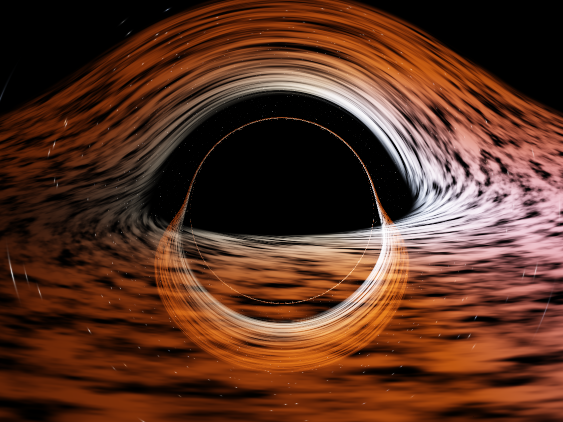
\includegraphics[width=0.243\textwidth]{figs/r_rk4_c.png} &
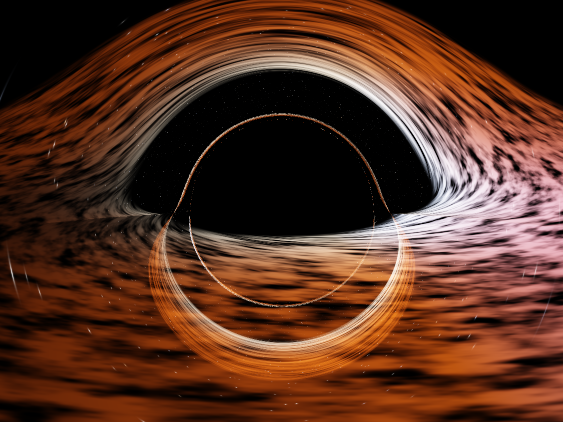
\includegraphics[width=0.243\textwidth]{figs/r_calibrada_c.png} &
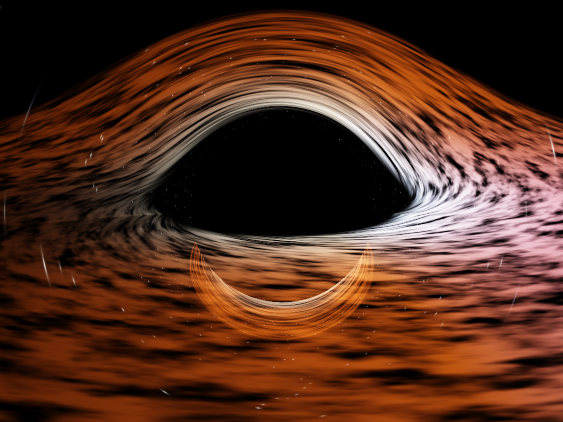
\includegraphics[width=0.243\textwidth]{figs/r_einstein_c.png} &
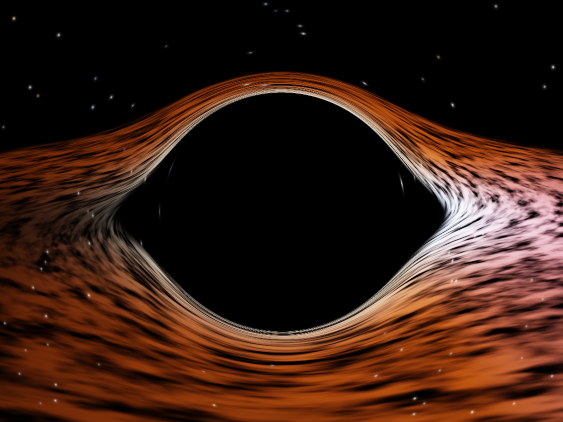
\includegraphics[width=0.243\textwidth]{figs/r_legado_c.png} \\
{\footnotesize (a) RK4} & {\footnotesize (b) calibrada} &
{\footnotesize (c) Einstein} & {\footnotesize (d) legada} \\[3pt]
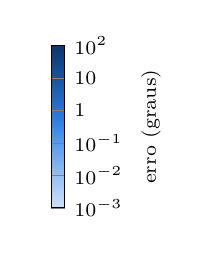
\begin{tikzpicture}
\begin{axis}[
  hide axis, scale only axis, width=1pt, height=0.170\textwidth,
  colormap={erro}{
    rgb255=(205,226,251) rgb255=(183,211,246) rgb255=(158,197,244)
    rgb255=(134,182,239) rgb255=(109,167,236) rgb255=(85,152,231)
    rgb255=(57,135,229)  rgb255=(42,120,214)  rgb255=(37,106,191)
    rgb255=(28,92,171)   rgb255=(24,79,149)   rgb255=(16,66,129)
    rgb255=(13,54,107)},
  colorbar, point meta min=-3, point meta max=2,
  colorbar style={height=0.170\textwidth, width=0.17cm,
    ytick={-3,-2,-1,0,1,2},
    yticklabels={$10^{-3}$,$10^{-2}$,$10^{-1}$,$1$,$10$,$10^{2}$},
    ylabel={erro (graus)},
    ticklabel style={font=\scriptsize}, ylabel style={font=\scriptsize}}]
\addplot [draw=none] coordinates {(0,0)};
\end{axis}
\end{tikzpicture} &
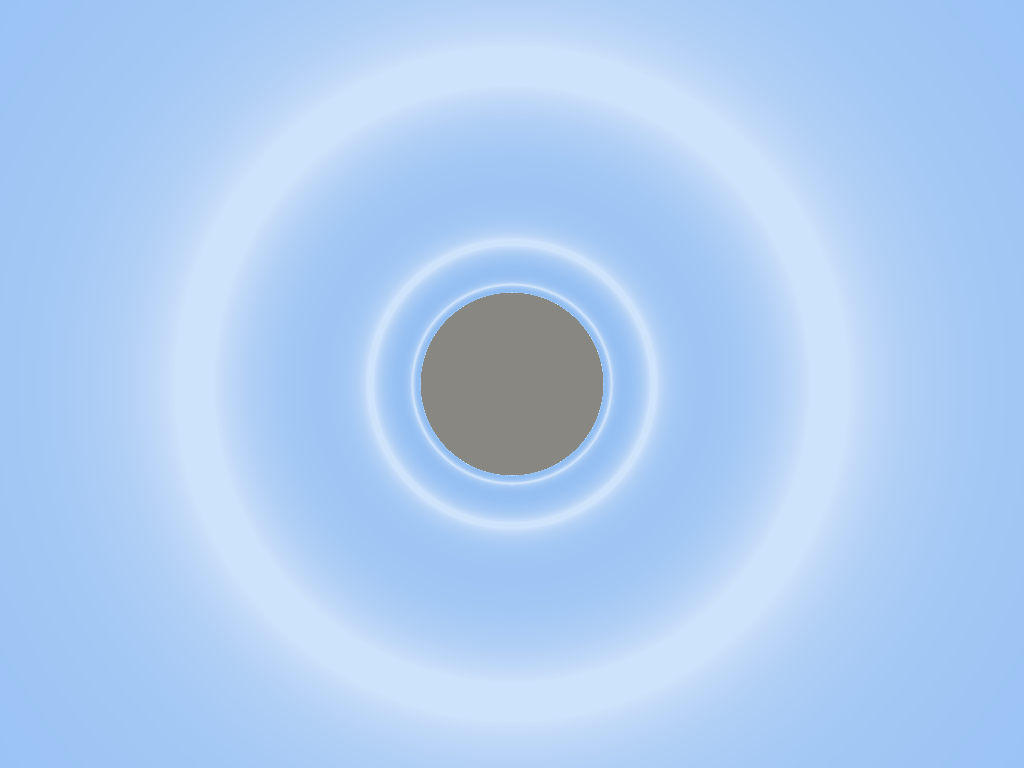
\includegraphics[width=0.243\textwidth]{figs/erro_calibrada.png} &
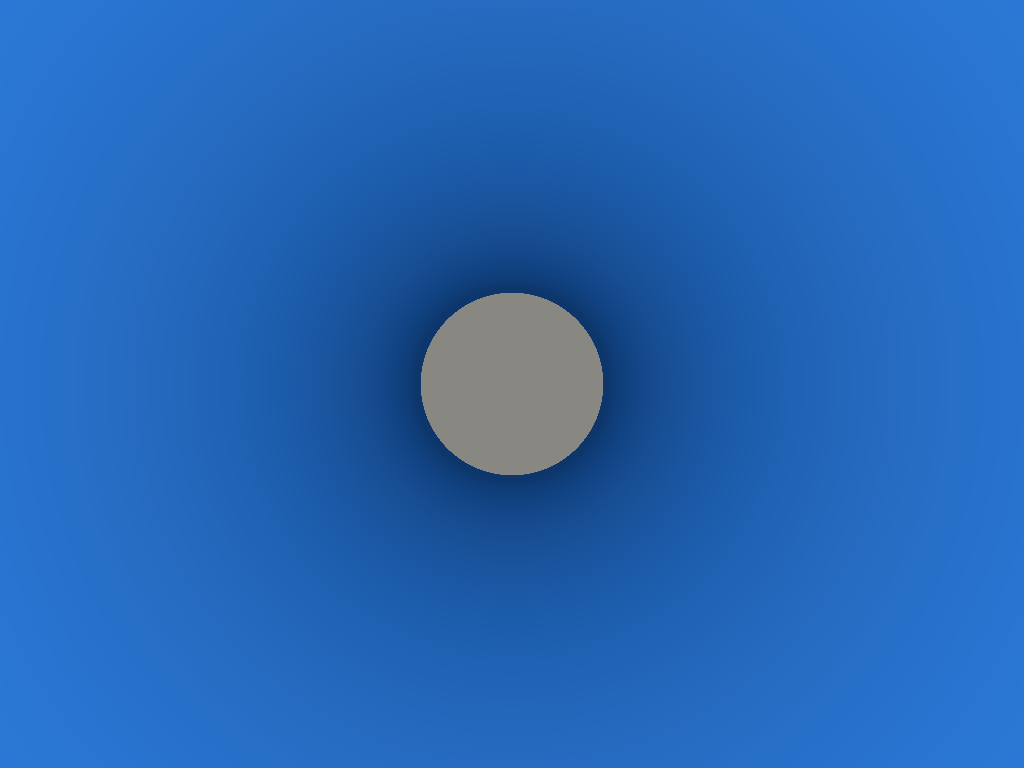
\includegraphics[width=0.243\textwidth]{figs/erro_einstein.png} &

\includegraphics[width=0.243\textwidth]{figs/erro_legado.png} \\
 & {\footnotesize (e) erro de (b)} & {\footnotesize (f) erro de (c)} &
{\footnotesize (g) erro de (d)}
\end{tabular}\\
{\footnotesize Fonte: elaborada pelos autores.}
\end{figure}

A Tabela~\ref{tab:resultados} e a linha inferior da
Figura~\ref{fig:comparacao} quantificam o erro. A heurística calibrada ficou em $0{,}004^\circ$, cerca de um quinze
avos de \emph{pixel} ($0{,}059^\circ$ nesta resolução), e manteve essa
ordem de grandeza a $10$ e $60\,R_s$, distâncias ausentes do ajuste. Os
anéis claros do painel (e) são os zeros do resíduo do ajuste. O maior
erro isolado, $0{,}84^\circ$ a $10\,R_s$, ocorre na borda da sombra,
onde $\alpha$ diverge e a própria referência em precisão simples perde
exatidão. A de Einstein só erra muito perto da sombra; a legada, em toda
a imagem.

\begin{table}[!ht]
\caption{Erro angular em relação ao RK4, em $1024\times768$, e tempo de
GPU por quadro em $1920\times1080$.}
\label{tab:resultados}
\centering
\begin{tabular}{lrrrrr}
\toprule
 & \multicolumn{3}{c}{\textbf{Erro médio (graus)}} & \textbf{p99} & \textbf{GPU} \\
\cmidrule(lr){2-4}
\textbf{Modelo} & $10\,R_s$ & $26\,R_s$ & $60\,R_s$ & $26\,R_s$ & \textbf{(ms)} \\
\midrule
Legada $1/r^2$    & 47,1   & 18,2   & 7,76   & 97,7   & 0,433 \\
Lente de Einstein & 29,0   & 5,63   & 1,33   & 65,8   & 0,559 \\
Lente calibrada   & 0,0045 & 0,0040 & 0,0071 & 0,0088 & 0,582 \\
RK4 (referência)  & ---    & ---    & ---    & ---    & 21,1  \\
\bottomrule
\end{tabular}
\caption*{\footnotesize Fonte: elaborada pelos autores.}
\end{table}


A Figura~\ref{fig:perfil} mostra que todos os custos crescem
linearmente com o número de \emph{pixels}. O RK4 cai abaixo de 60
quadros por segundo acima de cerca de $1{,}6$~Mpx e fica perto de 12
em 4K; a lente calibrada é 36 vezes mais barata e custa só 4\% mais que a
de Einstein, isto é, a precisão adicional sai praticamente de graça.

\begin{figure}[!ht]
\caption{Tempo de GPU por quadro em função da resolução, em escalas
logarítmicas. As linhas horizontais marcam 60 e 30 quadros por segundo.}
\label{fig:perfil}
\centering
\begin{tikzpicture}
\begin{axis}[
  width=0.74\textwidth, height=3.9cm,
  xmode=log, ymode=log,
  xmin=0.25, xmax=10, ymin=0.05, ymax=110,
  xtick={0.3072,0.9216,2.0736,3.6864,8.2944},
  xticklabels={480p,720p,1080p,1440p,2160p},
  ylabel={ms por quadro},
  tick label style={font=\footnotesize}, label style={font=\footnotesize},
  grid=major, major grid style={line width=0.2pt, draw=black!12},
  axis line style={draw=black!35},
  legend columns=4, legend style={at={(0.5,1.03)}, anchor=south,
    draw=none, font=\footnotesize, column sep=6pt},
  every axis plot/.append style={line width=1pt, mark size=1.8pt}]
\addplot [corRK,  mark=*]         table [x=mpx, y=rk4]       {dados/desempenho.dat};
\addlegendentry{RK4}
\addplot [corCal, mark=square*]   table [x=mpx, y=calibrada] {dados/desempenho.dat};
\addlegendentry{calibrada}
\addplot [corEin, mark=triangle*] table [x=mpx, y=einstein]  {dados/desempenho.dat};
\addlegendentry{Einstein}
\addplot [corLeg, mark=diamond*]  table [x=mpx, y=legado]    {dados/desempenho.dat};
\addlegendentry{legada}
\addplot [tintaMuda, line width=0.4pt, forget plot] coordinates {(0.25,16.67) (10,16.67)};
\addplot [tintaMuda, line width=0.4pt, forget plot] coordinates {(0.25,33.33) (10,33.33)};
\node [font=\scriptsize, text=tintaMuda, anchor=north west, inner sep=1.5pt] at (axis cs:0.26,16.67) {60 quadros/s};
\node [font=\scriptsize, text=tintaMuda, anchor=south west, inner sep=1.5pt] at (axis cs:0.26,33.33) {30 quadros/s};
\end{axis}
\end{tikzpicture}\\
{\footnotesize Fonte: elaborada pelos autores.}
\end{figure}

O resultado depende de o mapa ser unidimensional, e é isso que delimita
o método: rotação (Kerr) ou observador em movimento tornam o mapa
multidimensional, regime em que abordagens neurais
\cite{sun2025learning} se justificam. O erro do disco foi avaliado
apenas visualmente.

\section{Considerações Finais}

Isolar a curvatura forte em uma função de uma variável, aprendida por
mínimos quadrados da integração de referência, produziu uma heurística a
um quinze avos de \emph{pixel} da referência, que generaliza para
distâncias fora do ajuste e custa 36 vezes menos. Quando o mapa é
unidimensional, portanto, uma heurística calibrada substitui a
integração por \emph{pixel} sem perda visível. Ficam como trabalhos
futuros o erro do disco e observadores em movimento.

%%%%%%%%%%%%%%%%%%%%%%%%%% REFERÊNCIAS %%%%%%%%%%%%%%%%%%%%%%%%%%%%%%%%

\printbibliography

\end{document}
